\documentclass[10pt]{article}


\usepackage{times}
\usepackage{amsfonts}
\usepackage{amsmath}
\usepackage[psamsfonts]{amssymb}
\usepackage{latexsym}
\usepackage{color}
\usepackage{graphics}
\usepackage{enumerate}
\usepackage{amstext}
\usepackage{blkarray}
\usepackage{url}
\usepackage{epsfig}
\usepackage{bm}
\usepackage{hyperref}
\hypersetup{
    colorlinks=true,
    linkcolor=blue,
    filecolor=magenta,      
    urlcolor=blue,
}
\usepackage{mathtools}
\usepackage{minted}
 \usepackage{optidef}
 
\def\Kset{\mathbb{K}}
\def\Nset{\mathbb{N}}
\def\Qset{\mathbb{Q}}
\def\Rset{\mathbb{R}}
\def\Sset{\mathbb{S}}
\def\Zset{\mathbb{Z}}
\def\squareforqed{\hbox{\rlap{$\sqcap$}$\sqcup$}}
\def\qed{\ifmmode\squareforqed\else{\unskip\nobreak\hfil
\penalty50\hskip1em\null\nobreak\hfil\squareforqed
\parfillskip=0pt\finalhyphendemerits=0\endgraf}\fi}

\DeclareMathOperator*{\E}{\rm E}
\DeclareMathOperator*{\argmax}{\rm argmax}
\DeclareMathOperator*{\argmin}{\rm argmin}
\DeclareMathOperator{\sgn}{sign}
\DeclareMathOperator{\supp}{supp}
\DeclareMathOperator{\last}{last}
\DeclareMathOperator{\sign}{\sgn}
\DeclareMathOperator{\diag}{diag}
\providecommand{\abs}[1]{\lvert#1\rvert}
\providecommand{\norm}[1]{\lVert#1\rVert}
\def\vcdim{\textnormal{VCdim}}
\DeclareMathOperator*{\B}{\textbf{B}}
\DeclarePairedDelimiter\ceil{\lceil}{\rceil}
\DeclarePairedDelimiter\floor{\lfloor}{\rfloor}

\newcommand{\cX}{{\mathcal X}}
\newcommand{\cY}{{\mathcal Y}}
\newcommand{\cA}{{\mathcal A}}
\newcommand{\ignore}[1]{}
\newcommand{\bi}{\begin{itemize}}
\newcommand{\ei}{\end{itemize}}
\newcommand{\be}{\begin{enumerate}}
\newcommand{\ee}{\end{enumerate}}
\newcommand{\bd}{\begin{description}}
\newcommand{\ed}{\end{description}}
\newcommand{\h}{\widehat}
\newcommand{\e}{\epsilon}
\newcommand{\mat}[1]{{\mathbf #1}}
\newcommand{\R}{\mat{R}}
\newcommand{\0}{\mat{0}}
\newcommand{\M}{\mat{M}}

\newcommand{\SP}{\mathbf{S}_{+}^n}

\newcommand{\D}{\mat{D}}
\renewcommand{\r}{\mat{r}}
\newcommand{\x}{\mat{x}}
\renewcommand{\u}{\mat{u}}
\renewcommand{\v}{\mat{v}}
\newcommand{\w}{\mat{w}}
\renewcommand{\H}{\text{0}}
\newcommand{\T}{\text{1}}
\newcommand{\set}[1]{\{#1\}}
\newcommand{\xxi}{{\boldsymbol \xi}}
\newcommand{\ssigma}{{\boldsymbol \sigma}}
\newcommand{\Alpha}{{\boldsymbol \alpha}}
\newcommand{\tts}{\tt \small}
\newcommand{\hint}{\emph{hint}}
\newcommand{\matr}[1]{\bm{#1}}     % ISO complying version
\newcommand{\vect}[1]{\bm{#1}}     % ISO complying version

\newcommand{\Var}{\mathrm{Var}}
\newcommand{\Cov}{\mathrm{Cov}}

% New commands
\newcommand{\dom}{\textbf{dom}}
\newcommand{\epi}{\textbf{epi}}


\newenvironment{solution}{\vspace{.25cm}\noindent{\it Solution:}}{}

\begin{document}


\noindent MATH-GA.2012.001 Selected Topics in Numerical Analysis :\\
Convex and Nonsmooth Optimization, Spring 2020\\
Homework Assignment 3 \\
Yves Greatti - yg390\\

\be

	\item 
	\be
		\item $L(x, \nu) = \frac{1}{2} x^T Q x + \nu^T (A x - b)$
		
		\item $\nabla_x L(x,\nu) = Q x + A^T \nu$,  and $\nabla_x L(x,\nu) = 0 \Rightarrow x = -Q^{-1} A^T \nu$. For this minimizer $x$, the Lagrange dual function is: 
		$g(\nu) = \min_x L(x,\nu) = 
		 \frac{1}{2} (-Q^{-1} A^T \nu)^T Q (-Q^{-1} A^T \nu) + \nu^T A (-Q^{-1} A^T \nu) - \nu^T b$
		 $$g(\nu) = - \frac{1}{2} \nu^T A Q^{-1} A^T \nu -\nu^T b$$
		
		\item 
			$$\nabla_\nu  g(\nu) = -A Q^{-1} A^T \nu - b$$
			$$ \nabla_\nu  g(\nu) = 0 \Rightarrow \nu^* = - (A Q^{-1} A^T)^{-1} b$$
			The dual optimal value $d^*$ is:
			$$ d^* = g(\nu^*) = -\frac{1}{2} b^T [- (A Q^{-1} A^T)^{-1}]^T A Q^{-1}  A^T [- (A Q^{-1} A^T)^{-1}] b - b^T  [- (A Q^{-1} A^T)^{-1}]^T b $$
			$$ d^* = \frac{1}{2} b^T (A Q^{-1} A^T)^{-1} b$$
			
		\item The associated  $\hat{x}$ is:
			$$\hat{x} = -Q^{-1} A^T \nu^* =  -Q^{-1} A^T [- (A Q^{-1} A^T)^{-1} b] = Q^{-1} A^T  (A Q^{-1} A^T)^{-1} b$$
			
		\item $\hat{x}$ is feasible for the primal problem since it verifies the equality constraint $h(x) = A x - b = 0$ since $h(\hat{x}) = A Q^{-1} A^T  (A Q^{-1} A^T)^{-1} b - b = 0$.
		
		\item 
			$$f_0(\hat{x}) =  \frac{1}{2} \hat{x}^T \hat{x} = \frac{1}{2} b^T  (A Q^{-1} A^T)^{-1} A Q^{-1} Q  Q^{-1} A^T (A Q^{-1} A^T)^{-1} b$$
			$$f_0(\hat{x}) = \frac{1}{2} b^T    (A Q^{-1} A^T)^{-1}  b = p^* = d^*$$
		\item $d^* = p^*$ therefore there is no duality gap.
		
	\ee
	\item   BV Ex 5.1 
	 
	 \be
	 	\item Given $f_0(x) = x^2 +1$, the feasible set is the interval $[2,4]$. $f'_0(x) = 2 x$ so $f_0$ is increasing on  $[2,4]$, and the optimal value is $f_0(2)=5$ and the optimal solution is $2$.
		\item $$L(x,\lambda) = x^2 + 1 + \lambda (x-1) (x-4) = (\lambda + 1) x^2 -6 \lambda x + 1 + 8 \lambda$$
		The feasible set is indicated by the grey area between the two vertical lines at $x=2$ and $x=4$, $L(x,\lambda)$ is plotted for $\lambda=1,2,3$ (ref \ref{fig1}).
		We can verify on the graph that $\inf_x L(x, \lambda) \le p^*, p^*=5$. $L(x,\lambda)$ is convex (quadratic) and differentiable, we can set its gradient to zero to find its minimizer
		and write the Lagrange dual function $g(\nu)$. $\nabla_x L(x, \lambda) = 2 (\lambda+1) x - 6 \lambda$, $\nabla_x L(x, \lambda) = 0 \Rightarrow x = \frac{3 \lambda} {\lambda +1}$ for $\lambda \neq -1$. $g(\nu) = \inf_x  L(x, \lambda)$ is not bounded when $\lambda \le -1$ thus
		
		\[
		 g(\lambda)= \begin{dcases*}
			           \frac{- 9 \lambda^2}{\lambda + 1} + 1 + 8 \lambda & when $\lambda > -1$ \\
		        		   -\infty & otherwise
		\end{dcases*}
		\]
		
		\begin{figure}[H]
		\centering
			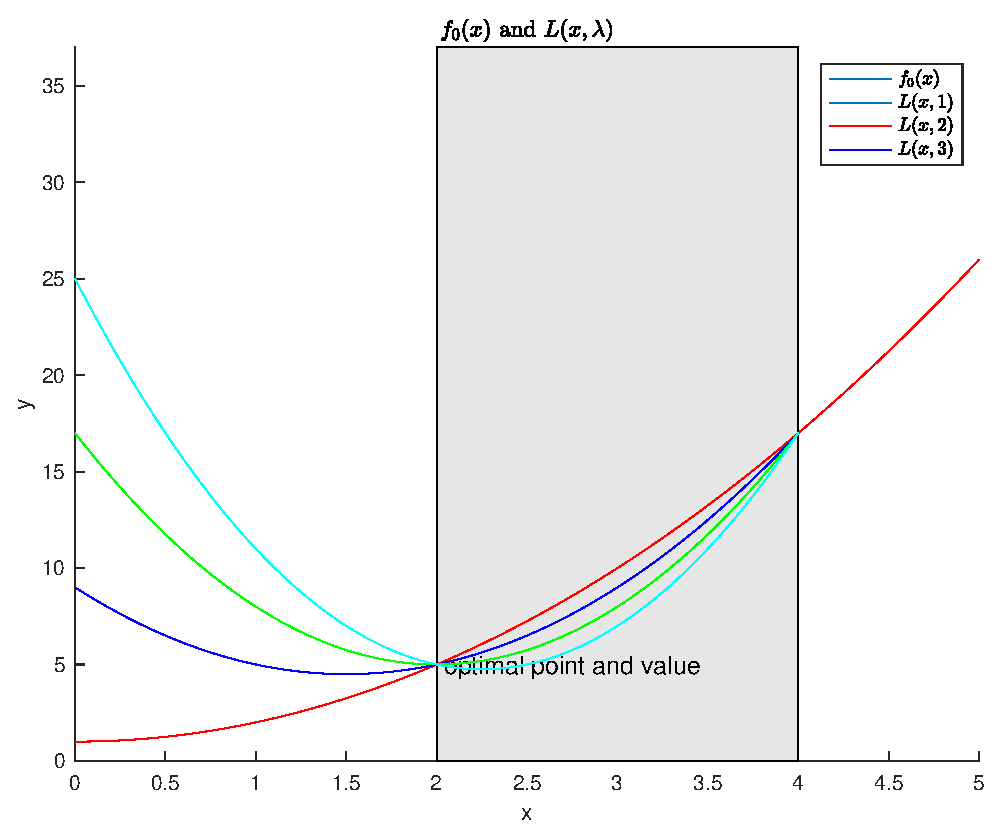
\includegraphics[width=200pt]{figures/simple_optimization_problem}
			\caption{Plot of $f_0$ and the Lagragian $L(x,\lambda)$ for $\lambda=1,2,3$.}
			\label{fig1}
		\end{figure}

		\begin{figure}[H]
		\centering
			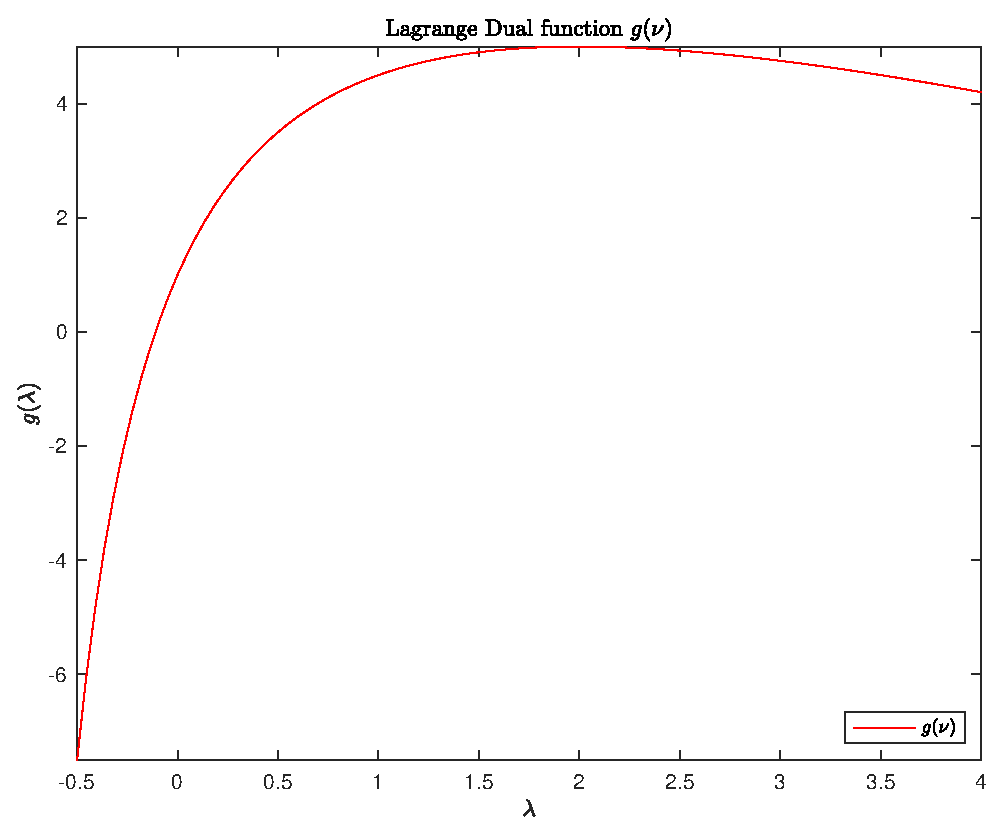
\includegraphics[width=200pt]{figures/simple_optimization_problem_dual}
			\caption{Plot of $g(\lambda)$ for $\lambda \in [-0.5, 5]$.}
			\label{fig2}
		\end{figure}
		
		\item The dual problem is:
		
		\begin{align*}
		 \text{ maximize } & g(\lambda) =  \frac{- 9 \lambda^2}{\lambda + 1} + 1 + 8 \lambda \\
		 \text{ subject to } & \lambda > -1
		\end{align*}
		
	 	Based on the graph of $g(\lambda)$, it is concave.
		Setting the derivative of $g(\lambda)$ to zero, leads to $g'(\lambda) = 8 - 9 \frac{\lambda (\lambda + 2)}{(\lambda + 1)^2} = 0$ which gives the dual optimal solution 
		$\lambda^*=2$ and the dual optimal value $d^* = 5 = p^*$ thus strong duality holds.
		
		\item Expanding $(x-2) (x-4) - u \le 0$, we have $x^2 -6 x + 8-u \le 0$. The determinant $\Delta = 4 (1+u)$ is valid only when $u \ge -1$ and the roots of the quadratic equation are
		$3 - \sqrt{1 + u}$ and $3 + \sqrt{1 + u}$, thus the feasible set is $[3 - \sqrt{1 + u}, 3 + \sqrt{1 + u}], u \ge -1$.
		We notice that $\min_x x^2  -6 x + 8 = -1$ and $p*(u)$ is not defined when $u <-1$. 
		And  for $p(u^*) = f(3 - \sqrt{1 + u}) = 11 + u - 6 \sqrt{1+u}$ reaches its global minimizer point
		 $u^*_0$ when $p'(u^*_0) = 1 - \frac{3}{\sqrt{1 + u}} = 0 \Rightarrow u^*_0 = 8, p(u^*_0) = 1$. 
		For $u \in [-1,8]$, the solution to the problem in x  is decreasing to the minimum value 1 to increase again when $u^* > 8$.
		
		\[
		 p(u^*)= \begin{dcases*}
			          \infty  			& when  	 $u < -1$ \\
			          11 + u - 6 \sqrt{1+u} & when	$u \in [-1,8]$ \\
		        		  1 				& when	$u > 8$
		\end{dcases*}
		\]
		We verify that $\frac{dp(u^*)} {du} = 1 - \frac{3} {\sqrt{1+u}}$ and $\frac{dp(0)} {du} = -2 = - \lambda^*$.
		
		\begin{figure}[H]
		\centering
			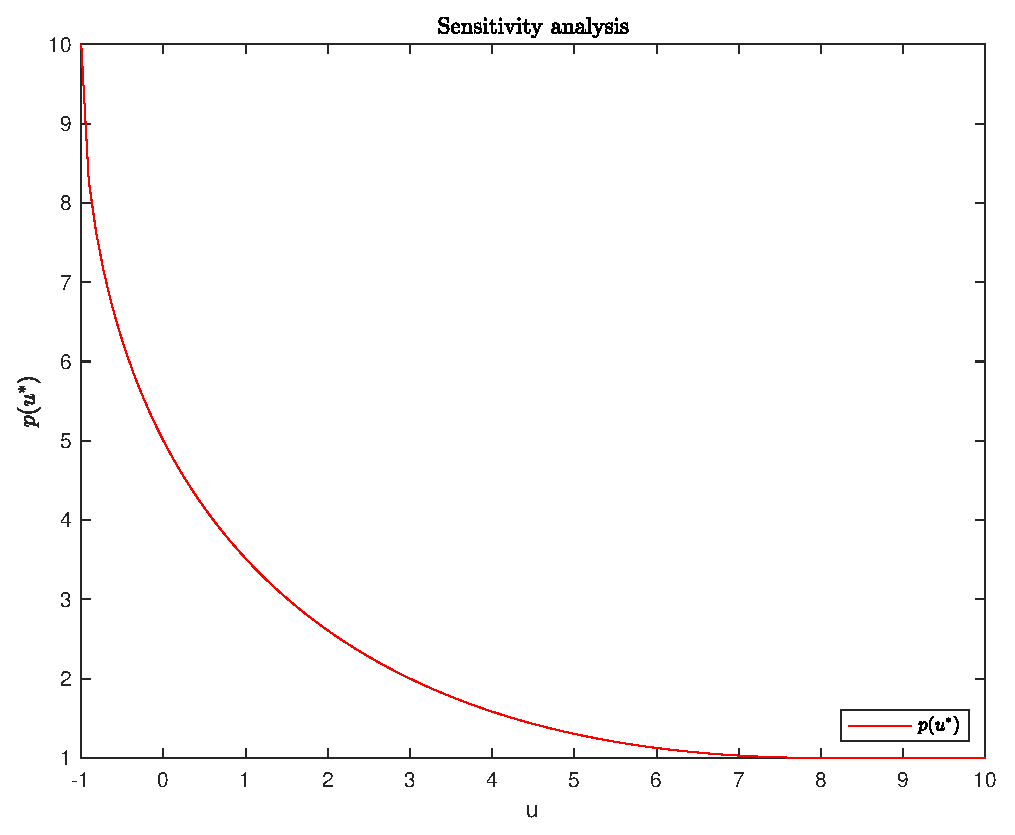
\includegraphics[width=200pt]{figures/sensitivity_analysis}
			\caption{$p(u^*)$.}
			\label{fig3}
		\end{figure}

	 \ee
	 
	  \item BV Ex 5.21
	  
	  \be
	  \item 
	  
	  The exponential function $e^{-x}$ is convex on $\mathbf{R}$, it then remains to determine if the Hessian of $f_1(x,y) = \frac{x^2}{y}$ is positive definite or semi definite.
	  $$ \nabla^2 f_1(x,y) =
	  \begin{bmatrix}
	  	 \frac{2}{y}	& 	\frac{-2x}{y^2} \\
	  	 \frac{-2x}{y^2}	& 	\frac{2x^2}{y^3} \\
	  \end{bmatrix}$$ 
	  The polynomial characteristic is $p(\lambda) = \frac{\lambda}{y^3} (y^3 \lambda - 2 (x^2 + y^2))$ so the eigenvalues are $0$ and $2 \frac{x^2 + y^2} {y^3} > 0, y > 0$. 
	  Hence the Hessian is positive semidefinite and $f_1(x,y)$ is convex. The problem is a convex optimization problem.
	  The minimizer of $e^{-x}$ satisfying the inequality constraint is $x=0$ and the optimal value is 1.
	  
	  \item The Lagrange dual function is $g(\lambda)=\inf_{x, y >0} (e^{-x} + \lambda \frac{x^2}{y})$
	  \[
		 g(\lambda)= \begin{dcases*}
			          0 			& when  	 $\lambda \ge 0$ \\
			          -\infty 		& when	 $\lambda < 0$
		\end{dcases*}
	\]
	The optimal value is $d^*  = 0$ for $\lambda^* \ge 0$, and the duality gap is $p^* - d^* = 1$.		 
	
	\item Since there is not strong duality, Slater's condition cannot hold.
	
	%\item If $u < 0$ the problem is not defined then $p(u^*) = \infty$, if $u=0, p(u^*) = 1$ and if $u > 0, p(u^*) = 0$ . We observe that $p(u^*)  \ge 1 - \lambda^* u$.
	
	\ee
\ee	

\end{document}
